\section{$N$+1-version Differential Testing}\label{sec:idea}
This section introduces the core concept of $N$+1-version differential testing with a
simple running example.  The overall structure consists of two
phases: a conformance test generation phase and a bug detection and localization
phase.

\begin{figure}[t]
  \centering
  \begin{subfigure}[t]{0.48\textwidth}
    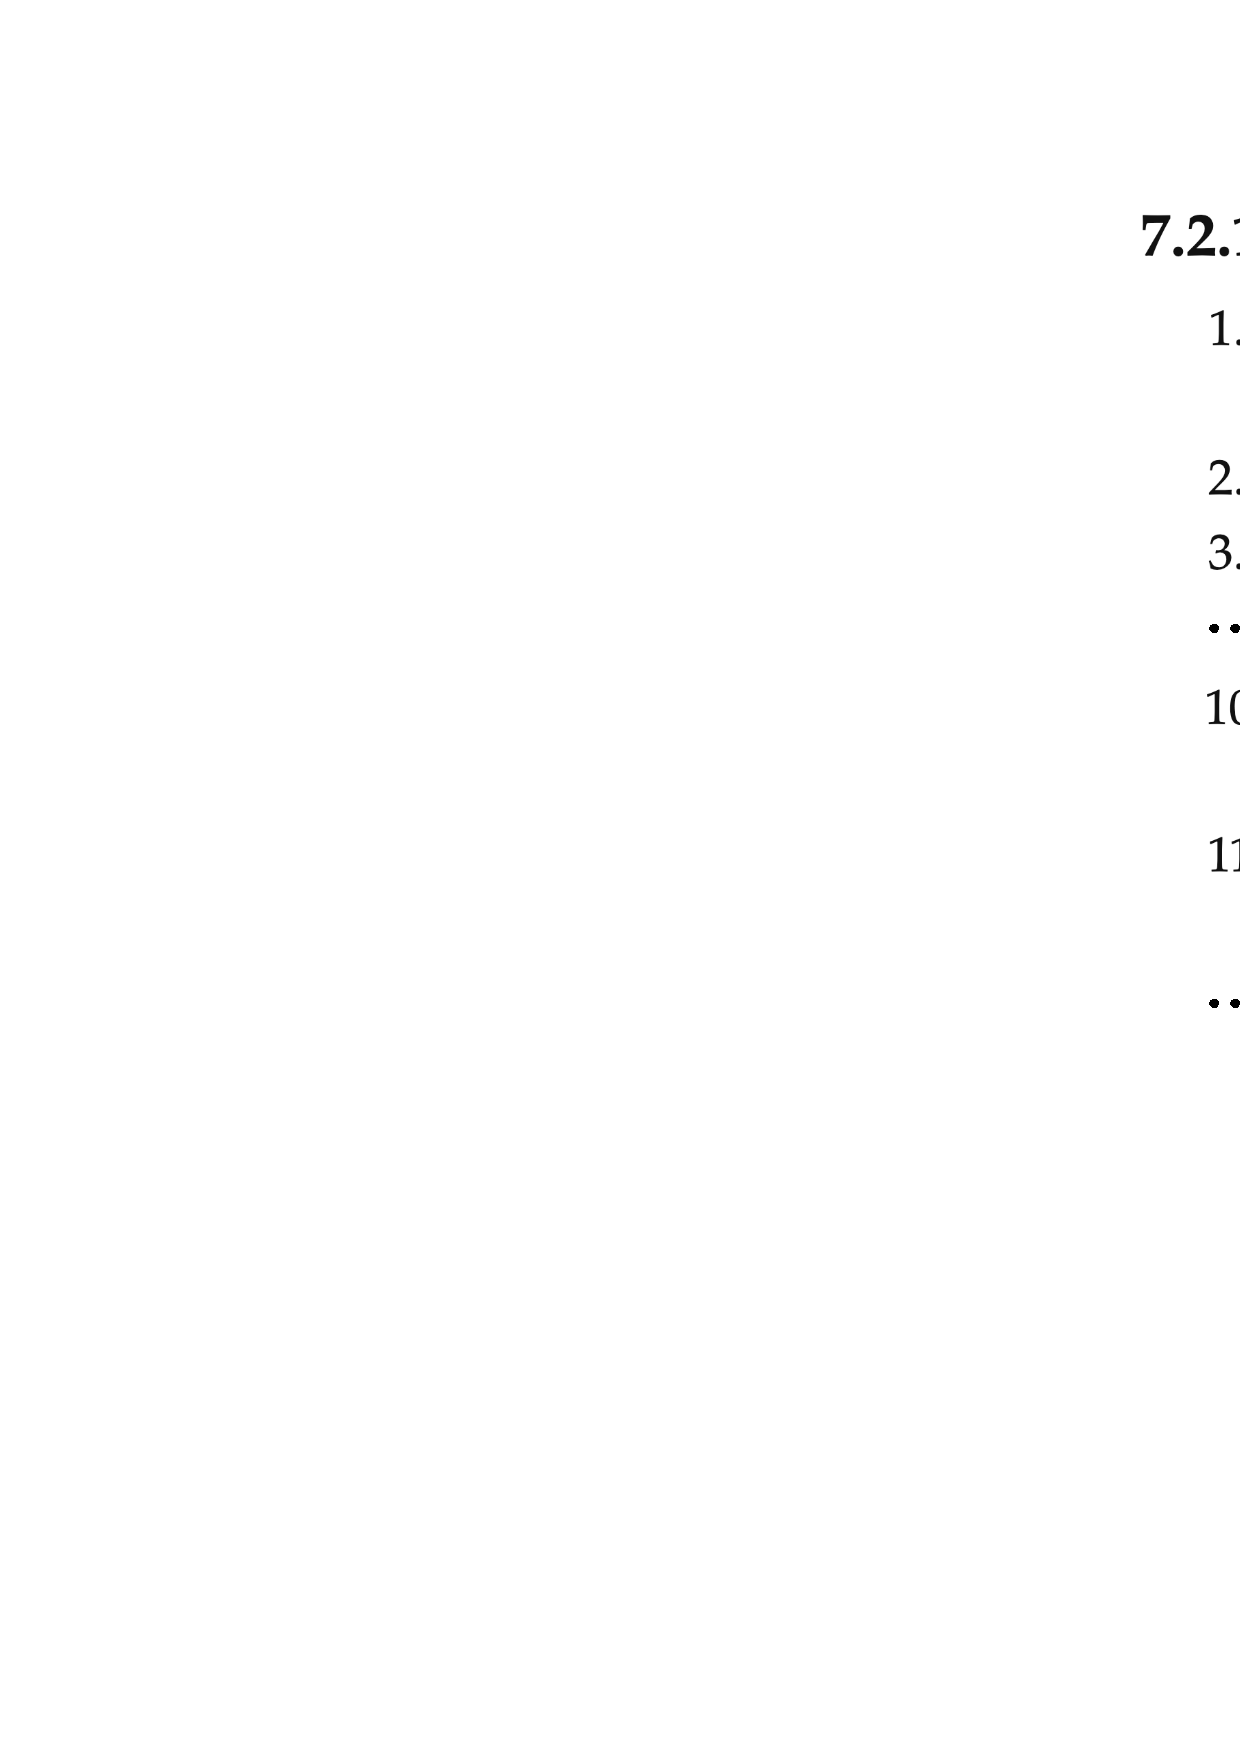
\includegraphics[width=\textwidth]{img/example-algo.pdf}
\vspace*{-.5em}
    \caption{The \textbf{Abstract Equality Comparison} abstract algorithm in
    ES11}
    \label{fig:example-algo}
  \end{subfigure}
  \begin{subfigure}[t]{0.43\textwidth}
    \begin{lstlisting}[style=myJSstyle]
// JavaScript engines: exception with "err"
// ECMAScript (ES11) : result === false
var obj = { valueOf: () => { throw "err"; } };
var result = 42 == obj;
    \end{lstlisting}
\vspace*{-.5em}
    \caption{JavaScript code using abstract equality comparison}
    \label{fig:example-js}
  \end{subfigure}
  \begin{subfigure}[t]{0.45\textwidth}
    \begin{lstlisting}[style=myJSstyle]
try {
  var obj = { valueOf: () => { throw "err"; } };
  var result = 42 == obj;
  assert(result === false);
} catch (e) {
  assert(false);
}
    \end{lstlisting}
\vspace*{-1em}
    \caption{JavaScript code with injected assertions}
    \label{fig:example-injected}
  \end{subfigure}
  \caption{Abstract algorithm in ES11 and code example using it}
  \label{fig:example}
  \vspace*{-1em}
\end{figure}


\subsection{Main Idea}

Differential testing utilizes the cross-referencing oracle, which is
an assumption that any discrepancies between program behaviors on the same input
could be bugs.  It compares the execution results of a program with the same
input on $N$ different implementations.  When an implementation produces a different
result from the one by the majority of the implementations, differential testing
reports that the implementation may have a bug.

On the contrary, $N$+1-version differential testing utilizes not only the cross-referencing oracle
using multiple implementations but also a mechanized specification.  It first
generates test code from a mechanized specification, and tests 
$N$ different implementations of the specification using the generated test code
as in differential testing.  In addition, it can detect possible bugs in the specification
as well when most implementations fail for a test.  In such cases,
because a bug in the specification could be triggered by the test, it
localizes the bug using statistical information as we explain later in this section.

\begin{figure*}[t]
  \centering
  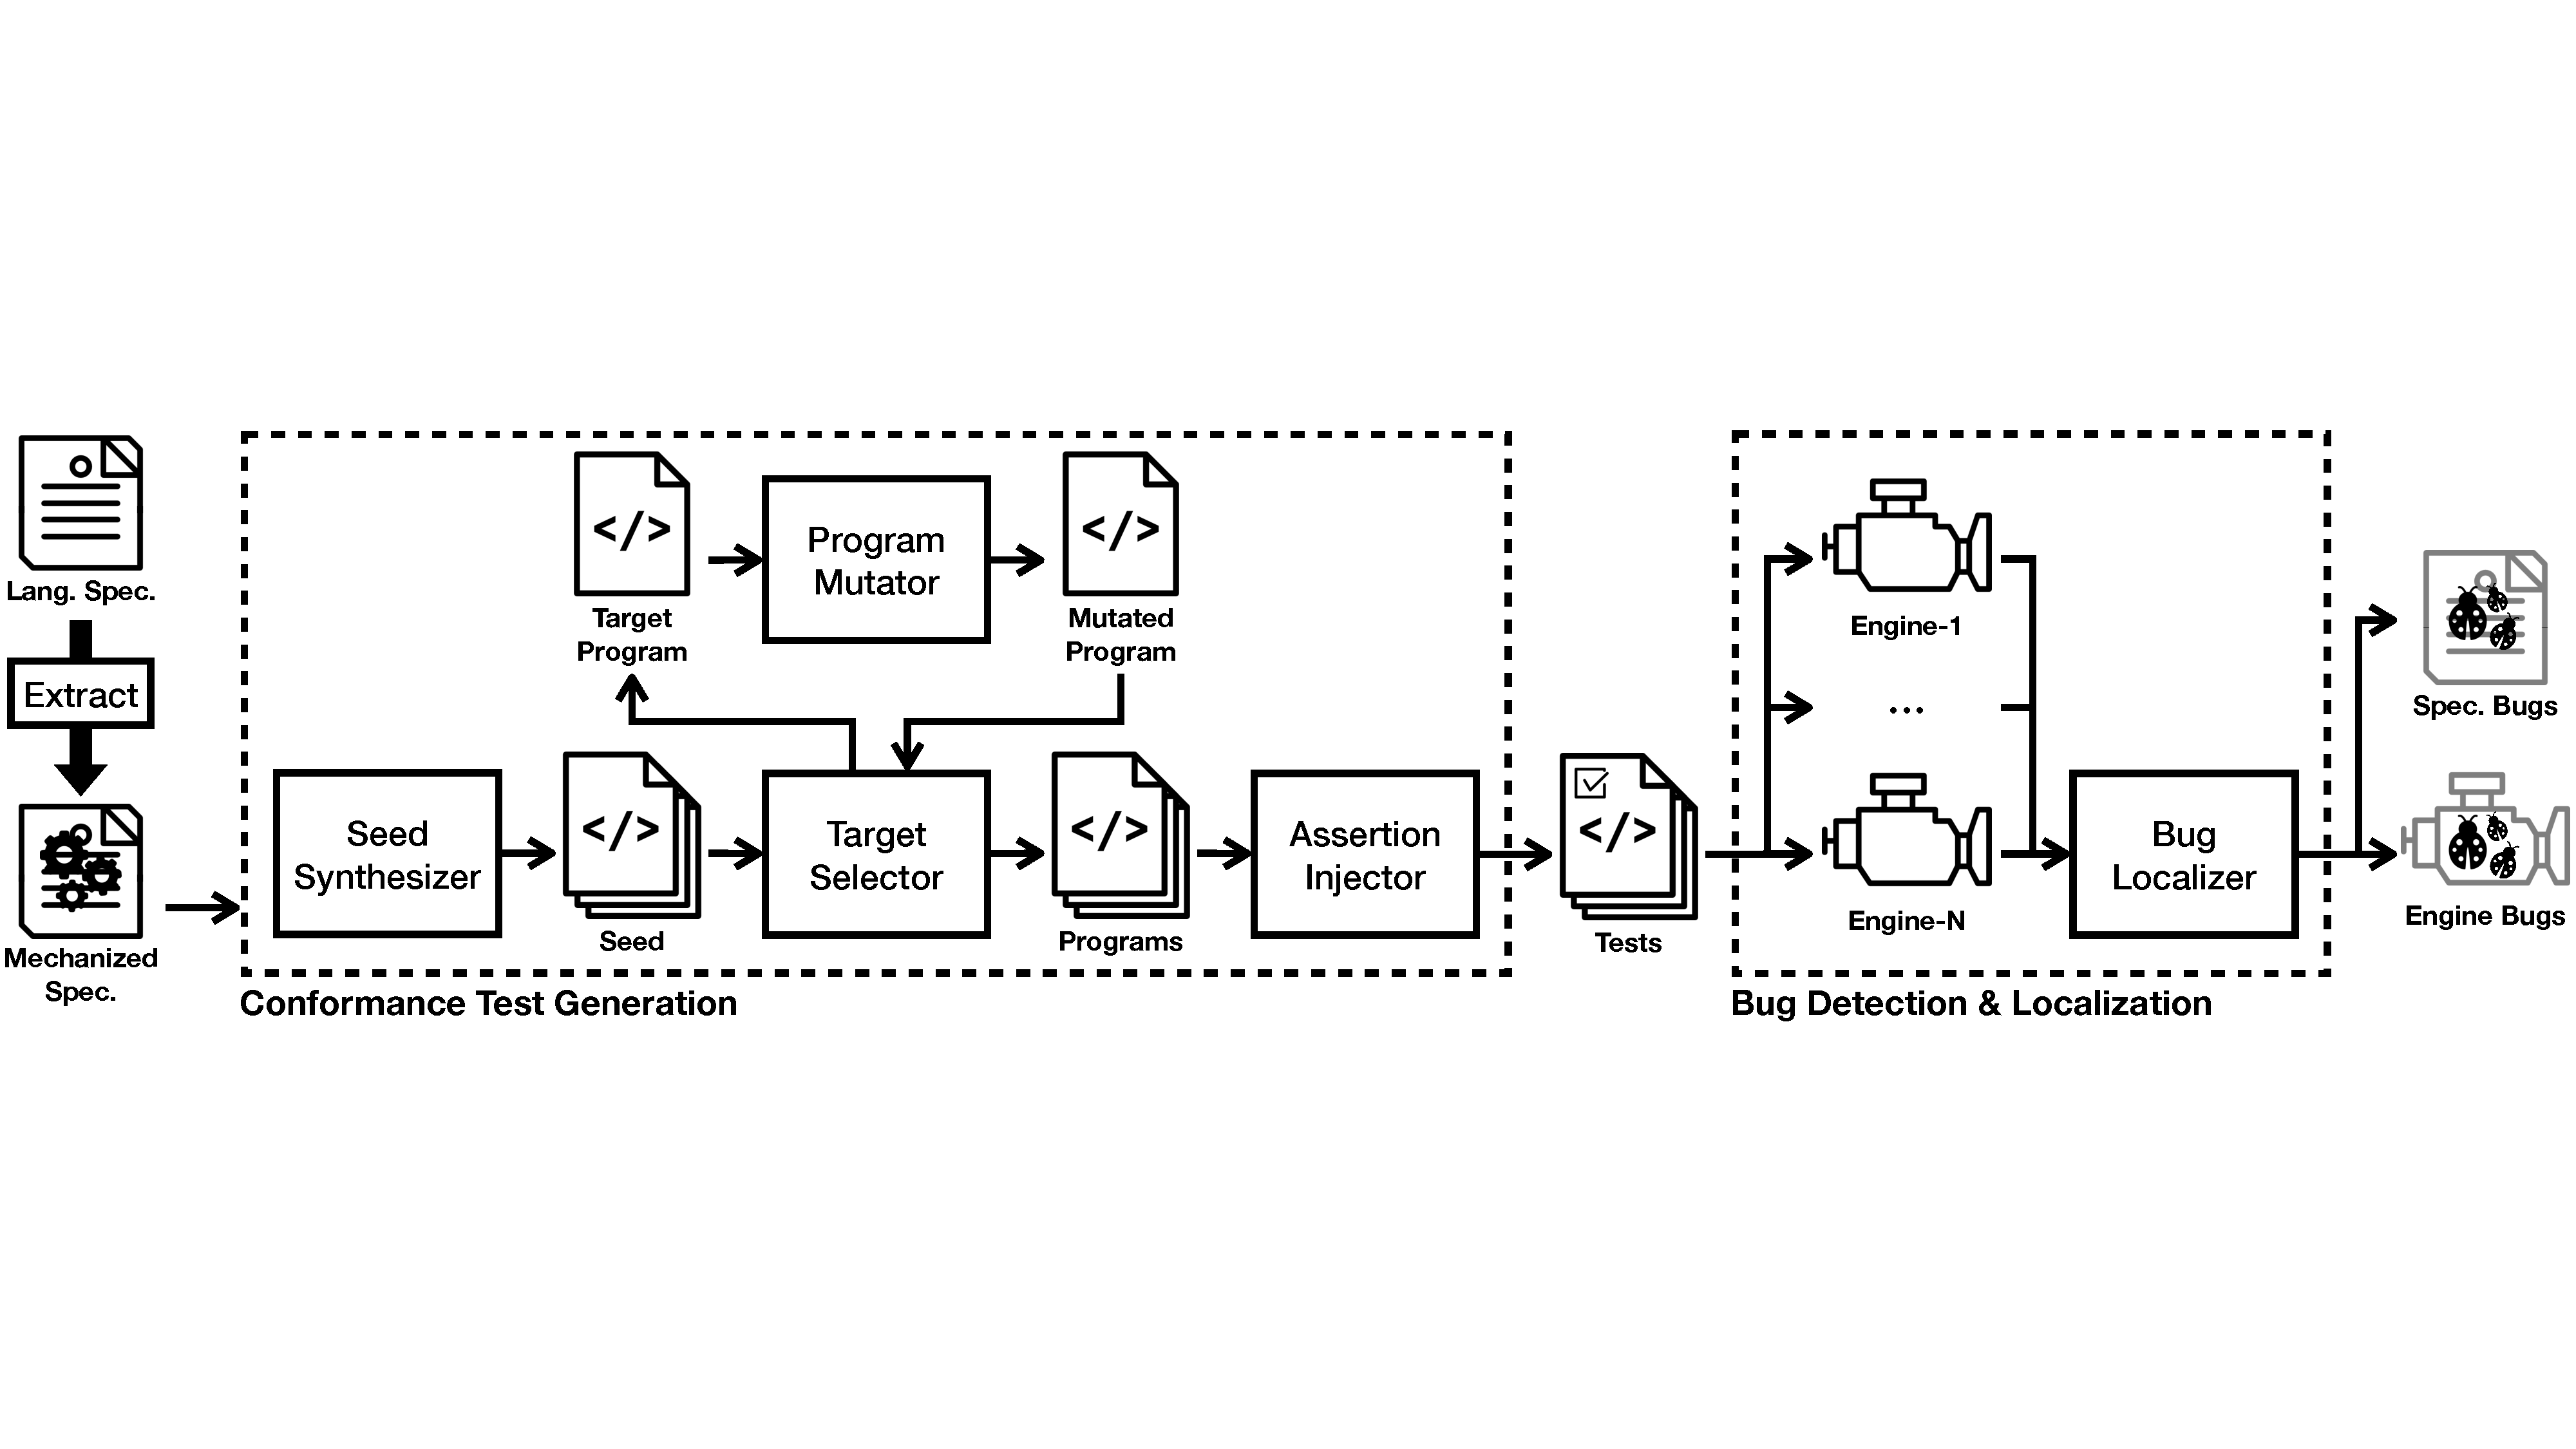
\includegraphics[width=0.98\textwidth]{img/overall.pdf}
  \vspace*{.5em}
  \caption{Overall structure of $N$+1-version differential testing for $N$
    implementations (engines) and one language specification}
  \label{fig:overall}
  \vspace*{-1em}
\end{figure*}


\subsection{Running Example}

We explain how $N$+1-version differential testing works with a simple
JavaScript example shown in Figure~\ref{fig:example}.

Figure~\ref{fig:example}(a) is an excerpt from ECMAScript 2020 (ES11),
which shows some part of the \textbf{Abstract Equality Comparison} abstract algorithm.
It describes the semantics of non-strict equality comparison such as \code{==} and \code{\!=}.
For example, $\code{null == undefined}$ is $\code{true}$ because of
the algorithm step 2.  According to the steps 10 and 11, if the type of a value is
String, Number, BigInt, or Symbol, and the type of the other value is Object, the algorithm calls
\textbf{ToPrimitive} to convert the JavaScript object to a primitive value.
Note that this is a specification bug caused by unhandled abrupt completions!
To express control diverters such as exceptions, $\code{break}$, $\code{continue}$,
$\code{return}$, and $\code{throw}$ statements in addition to normal values,
ECMAScript uses ``abrupt completions''.  To denote necessary checking of them,
ECMAScript annotates the question mark prefix (?) to all function calls possible
to return abrupt completions.  However, even though \textbf{ToPrimitive} can
produce an abrupt completion, the calls of \textbf{ToPrimitive} in steps 10 and
11 do not use the question mark, which is a bug.

Now, let's see how $N$+1-version differential testing can detect the
bug in the specification. Consider the example JavaScript code in
Figure~\ref{fig:example}(b), which triggers the above specification bug.
In the \textbf{Abstract Equality Comparison} algorithm, variables
\textit{x} and \textit{y} respectively denote $\code{42}$ and an object with a property
named $\code{valueOf}$ whose value is a function throwing an error.
Step 10 calls \textbf{ToPrimitive} with the object as its argument, and the call returns
an abrupt completion because the call of $\code{valueOf}$ throws an error.
However, because the call of \textbf{ToPrimitive} in step 10 does not
use the question mark, the specification semantics silently ignores the abrupt completion and
returns $\code{false}$ as the result of comparison. Using the specification semantics,
we can inject assertions to check that the code does not throw any errors as shown
in Figure~\ref{fig:example}(c). Then, by running the code with the injected assertions
on $N$ JavaScript engines, which throw errors, we can find that the specification
may have a bug.  Moreover, we can localize the bug using statistical information:
because most conformance tests that go through steps 10 and 11 of the algorithm
would fail in most of JavaScript engines, we can use the information
to localize the bug in the steps 10 and 11 of \textbf{Abstract
Equality Comparison} with high probability.


\subsection{Overall Structure}

Figure~\ref{fig:overall} depicts the overall structure of $N$+1-version differential testing
for $N$ different implementations (engines) and one language specification.
It takes a mechanized specification extracted from a given language
specification, it first performs the conformance test generation phase, which
automatically generates conformance tests that reflect the language
syntax and semantics described in the specification.  Then, it performs the
bug detection and localization phase, which detects and localizes bugs
in the engines or the specification by comparing the results
of the generated tests on $N$ engines.

The functionalities of each module in the overall structure are as follows:

\subsubsection{Seed Synthesizer}
The first module of the conformance test generation phase is \mytextsf{Seed Synthesizer},
which synthesizes an initial seed programs using the language syntax.
Its main goal is to synthesize (1) a few number of
(2) small-sized programs (3) that cover possible cases in the syntax rules as many as possible.

\subsubsection{Target Selector}
Starting from the seed programs generated by \mytextsf{Seed Synthesizer}
as the initial \emph{program pool}, \mytextsf{Target Selector}
selects a target program in the program pool that potentially increases the
coverage of the language semantics by the pool.
From the selected target program, \mytextsf{Program Mutator} constructs a new mutated program
and adds it to the program pool.  When specific criteria, such as an iteration limit, are satisfied,
\mytextsf{Target Selector} stops selecting target programs and returns
the program pool as its result.

\subsubsection{Program Mutator}
The main goal of \mytextsf{Program Mutator} is to generate a new program by
mutating a given target program in order to increase the coverage of
the language semantics by the program pool.
If it fails to generate a new program to increase the semantics coverage,
\mytextsf{Target Selector} retries to select a new target program and repeats this
process less than a pre-defined iteration limit.

\subsubsection{Assertion Injector}
Finally, the conformance test generation phase modifies the programs in the pool to generate
conformance tests by injecting appropriate assertions reflecting the
semantics described in the specification.  More specifically,
\mytextsf{Assertion Injector} executes each program in the pool on the mechanized
specification and obtains the final state of its execution.  It then
automatically injects assertions to the program using the final state.

\subsubsection{Bug Localizer}
Then, the second phase executes the conformance tests on $N$ engines and
collects their results.  For each test, if a small number of engines fail,
it reports potential bugs in the engines that fail the test.
Otherwise, it reports potential bugs in the specification.
In addition, its \mytextsf{Bug Localizer} module uses \textit{Spectrum
Based Fault Localization} (SBFL)~\cite{sbfl-survey}, a localization
technique utilizing the coverage and pass/fail results of test cases, to
localize potential bugs.
